% #######################################
% ########### FILL THESE IN #############
% #######################################
\def\mytitle{Implementation of Boolean Logic \\using OR and Inverter Gates}
\def\mykeywords{}
\def\myauthor{G Kumar}
\def\contact{kumargandhamaneni20016@gmail.com}
\def\mymodule{Future Wireless Communication(FWC22080)}
% #######################################
% #### YOU DON'T NEED TO TOUCH BELOW ####
% #######################################
\documentclass[10pt, a4paper]{article}
\usepackage[a4paper,outer=1.5cm,inner=1.5cm,top=1.75cm,bottom=1.5cm]{geometry}
\twocolumn
\usepackage{graphicx}
\usepackage{circuitikz}
\usetikzlibrary{calc}
\graphicspath{{./images/}}
%colour our links, remove weird boxes
\usepackage[colorlinks,linkcolor={black},citecolor={blue!80!black},urlcolor={blue!80!black}]{hyperref}
\usetikzlibrary{arrows,shapes.gates.logic.US,shapes.gates.logic.IEC,calc}
%Stop indentation on new paragraphs
\usepackage[parfill]{parskip}
%% Arial-like font
\usepackage{lmodern}
\renewcommand*\familydefault{\sfdefault}
%Napier logo top right
\usepackage{watermark}
%Lorem Ipusm dolor please don't leave any in you final report ;)
\usepackage{lipsum}
\usepackage{xcolor}
\usepackage{listings}
%give us the Capital H that we all know and love
\usepackage{float}
%tone down the line spacing after section titles
\usepackage{titlesec}
%Cool maths printing
\usepackage{amsmath}
%PseudoCode
\usepackage{algorithm2e}
\usepackage{circuitikz}

\titlespacing{\subsection}{0pt}{\parskip}{-3pt}
\titlespacing{\subsubsection}{0pt}{\parskip}{-\parskip}
\titlespacing{\paragraph}{0pt}{\parskip}{\parskip}
\newcommand{\figuremacro}[5]{
    \begin{figure}[#1]
        \centering
        \includegraphics[width=#5\columnwidth]{#2}
        \caption[#3]{\textbf{#3}#4}
        \label{figure:#2}
    \end{figure}
}

\lstset{
frame=single, 
breaklines=true,
columns=fullflexible
}

\thiswatermark{\centering \put(0,-90.0){
\includegraphics[scale=0.2]{iith}} }
\title{\mytitle}
\author{\myauthor\hspace{1em}\\\contact\\IITH\hspace{0.5em}-\hspace{0.5em}\mymodule}
\date{}
\hypersetup{pdfauthor=\myauthor,pdftitle=\mytitle,pdfkeywords=\mykeywords}
\sloppy
% #######################################
% ########### START FROM HERE ###########
% #######################################
\usepackage{tabularx}
\begin{document}
	\maketitle
	\tableofcontents
	\begin{abstract}
	    %Replace the lipsum command with actual text 
		This manual shows how to implement Boolean Logic with OR and Inverter Gates through 7447 BCD-Seven Segment Display Decoder
	\end{abstract}
    \section{Introduction}
    There are many different ways to implement a Boolean Logic through different Gates.In this manual, we implement the Boolean expression, F=xy+x'y'+y'z using OR and Inverter Gates.
	\section{Components}
	
\begin{table}[htbp]
 \begin{center}
    \begin{tabular}{|l|c|c|c|c|c|c} \hline \textbf{Component}
  & \textbf{value} & \textbf{quantity} \\
 \hline
Resistor & 220 ohm & 1 \\ \hline
Arduino & UNO & 1 \\ \hline
decoder & 7447 & 1  \\ \hline
Jumper wires & M-M & 20\\ \hline
sevensegment display &  & 1 \\ \hline
Bread board &  & 1 \\ \hline
\end{tabular}   
\end{center}
\caption{\label{table:table} }
\end{table}
	\section{Hardware}
	\textbf{3.1}
    Connection between the sevensegment display and 7447 IC in Figure 1 using Table 2.
    \begin{center}
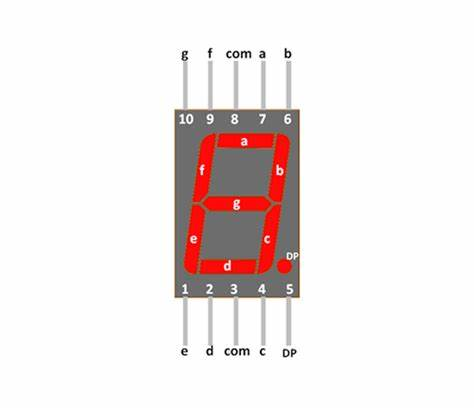
\includegraphics[scale=.20]{sevenseg.jpg}
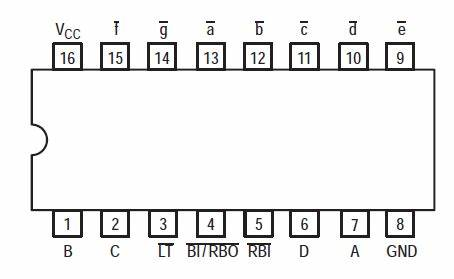
\includegraphics[scale=.20]{7447ic.jpg}
\end{center}
Figure 1:Sevensegment and 7447 IC.
	\begin{table}[htbp]
    \begin{center}
    \begin{tabular}{|l|c|c|c|c|c|c|c|c} \hline \textbf{7447}
  & a' & b' & c' & d' & e' & f' & g' \\
 \hline
\textbf{Display} & a & b & c & d & e & f & g \\ \hline
\end{tabular}   
\end{center}
\caption{\label{table:dummytable} }
\end{table}
\\	\textbf{3.2}
	connection of lower pins of 7447 IC to the Arduino according to Table 3 and connecting VCC,GND of IC to 5V,GND of Arduino respectively.
		\begin{table}[htbp]
    \begin{center}
    \begin{tabular}{|l|c|c|c|c|c|c|c|c} \hline \textbf{7447}
  & D & C & B & A \\
 \hline
\textbf{Arduino} & 5 & 4 & 3 & 2\\ \hline
\end{tabular}   
\end{center}
\caption{\label{table:dummytable} }
\end{table}
\\\textbf{3.3}
Finally, Giving 1 as input to the arduino through making the connections in table 4.
	\begin{table}[htbp]
    \begin{center}
    \begin{tabular}{|l|c|c|c|c|} \hline 
  & X & Y & Z \\
 \hline
\textbf{Input} & 0 & 0 & 1 \\ \hline
\textbf{Arduino} & 8 & 7 & 6\\ \hline
\end{tabular}   
\end{center}
\caption{\label{table:dummytable} }
\end{table}
\section{Implementation}
\textbf{4.1}
By making Logic circuit for the Boolean Logic, F=xy+x'y'+y'z,we get the circuit as in figure 2.
And the thruth table for the circuit is given in Table 5.

\textbf{4.2}
The code below realizes the Boolean Logic for F in table 5.
\begin{lstlisting}
 https://github.com/kumarg9999/IITH_FWC/blob/main/Assignment1/codes/boolexp.txt
\end{lstlisting}
\begin{circuitikz} \draw
%\usetikzlibrary{arrows,shapes.gates.logic.US,shapes.gates.logic.IEC,calc}
(0,4) node[or port]  (or1) {}
(0,2) node[or port]  (or2) {}
(0,0) node[or port] (or3) {}
(2,0) node[not port] (not1) {}
(2,2) node[not port] (not2) {}
(2,4) node[not port] (not3) {}
(6,2) node[or port, number inputs=3] (or4) {}

(or1.out) -- (not3.in)
(or2.out) -- (not2.in)
(or3.out) -- (not1.in)
(not1.out) -- (or4.in 3)
(not2.out) -- (or4.in 2)
(not3.out) -- (or4.in 1);
\node[left] at (or1.in 1) {\(X\)};
\node[left] at (or1.in 2) {\(Y\)};
\node[left] at (or1.in 1)[ocirc] {};
\node[left] at (or1.in 2) [ocirc] {};
\node[left] at (or2.in 1) {\(X\)};
\node[left] at (or2.in 2) {\(Y\)};
\node[left] at (or3.in 2) [ocirc] {};
\node[left] at (or3.in 1) {\(Y\)};
\node[left] at (or3.in 2) {\(Z\)};
\end{circuitikz}
\begin{center}
    Figure 2
\end{center}
 \begin{tabularx}{0.45\textwidth} { 
  | >{\centering\arraybackslash}X 
  | >{\centering\arraybackslash}X
  | >{\centering\arraybackslash}X
  | >{\centering\arraybackslash}X
  | >{\centering\arraybackslash}X
  | >{\centering\arraybackslash}X 
  | >{\centering\arraybackslash}X
  | >{\centering\arraybackslash}X | }
\hline
 \textbf{X} & \textbf{Y} & \textbf{Z} &\textbf{F}& \textbf{D}&\textbf{C}&\textbf{B}&\textbf{A} \\ \hline
0&0&1&1&0&0&0&1 \\ \hline
0&1&0&1&0&0&0&1 \\ \hline
0&0&0&0&0&0&0&0 \\ \hline
0&1&1&0&0&0&0&0 \\ \hline
1&0&0&0&0&0&0&0 \\ \hline
1&0&1&1&0&0&0&1 \\ \hline
1&1&0&1&0&0&0&1 \\ \hline
1&1&1&1&0&0&0&1 \\ \hline
\end{tabularx}   
\end{document}